\def\stitle{\theexercise\ - Anweisungen 2}
\section{\stitle}
\begin{frame}
    \frametitle{\stitle}
\tableofcontents[current]    
\end{frame}

\begin{frame}[t]%
    \frametitle{\stitle}

Gegeben sei der folgende Ausschnitt eines Java-Programms.
\lstinputlisting[style=JAVAsmalllines]{\getexercisefolder/Anweis2.java}

\begin{itemize}
\item[(a)] Welcher Buchstabe wird auf dem Bildschirm ausgegeben, falls \code{i} den Wert $1$, $2$, $3$ bzw. $4$ besitzt?
\end{itemize}
\end{frame}


\begin{frame}[fragile]%
 \frametitle{a) Strukturprogramm mit Java-Editor}%

\begin{center}
\lstinputlisting[style=JAVAlines]{\getexercisefolder/Anweis2_snippet.java}
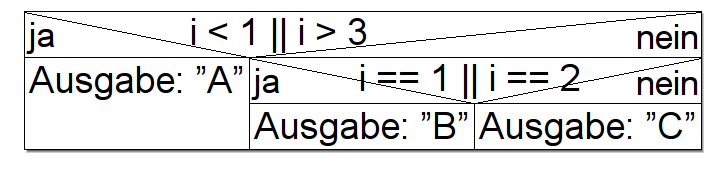
\includegraphics[width=1\textwidth]{\getexercisefolder/Bilder/Struktogramm_a}
\end{center}
\end{frame}
